\chapter{PROBLEM DEFINITION AND RESEARCH QUESTIONS}

% ================================================
% 3.1 Introduction
% ================================================
\section{Introduction}

This chapter formalizes the research problem addressed by this thesis. Based on empirical analysis of the NYC Yellow Taxi dataset, we identify critical gaps in existing streaming DQ frameworks and derive research questions that guide the rest of this work.

% ================================================
% 3.2 Case Study: NYC Yellow Taxi Dataset
% ================================================
\section{Case Study: NYC Yellow Taxi Dataset}

We use the NYC Yellow Taxi dataset as our case study. The dataset is published by the NYC Taxi and Limousine Commission (TLC) and contains trip records for all yellow medallion taxis. We analyze 3,076,903 records from July 2024, with temporal validation across 26 months (January 2024 -- February 2026).

\subsection{Dataset Schema}

The dataset contains 19 raw columns plus 4 derived features computed during preprocessing. Key columns include:

\begin{itemize}
    \item \textbf{VendorID:} Integer identifier for the TPEP provider (1=CMT, 2=VTS, 6=Unknown).
    \item \textbf{tpep\_pickup\_datetime / tpep\_dropoff\_datetime:} Pickup and dropoff timestamps.
    \item \textbf{passenger\_count:} Number of passengers (NULL indicates a completeness violation).
    \item \textbf{trip\_distance:} Trip distance in miles (must be $> 0$).
    \item \textbf{RatecodeID:} Rate category (1=Standard, 2=JFK, 3=Newark, 4=Negotiated, 5=Group, 6=Shared, 99=Unknown). This is the key context dimension for CA-DQStream.
    \item \textbf{PULocationID / DOLocationID:} Taxi zone identifiers for pickup and dropoff.
    \item \textbf{payment\_type:} 1=Card, 2=Cash, 3=No charge, 4=Dispute, 5=Unknown, 6=Voided.
    \item \textbf{fare\_amount, total\_amount:} Dollar values for fare and total charges.
    \item \textbf{tip\_amount:} Tip amount (only non-zero for card payments, payment\_type$=1$).
\end{itemize}

Derived features include \texttt{duration\_min} (dropoff minus pickup in minutes), \texttt{speed\_mph} (trip distance divided by duration in hours, clipped at 100 mph), and time slot bins derived from pickup hour.

\subsection{Data Volume and Temporal Coverage}

CA-DQStream uses NYC Taxi data from January 2024 through February 2026:

\begin{itemize}
    \item \textbf{Training (Baseline):} January 2024, 2,964,624 records.
    \item \textbf{Primary Test:} July 2024, 3,076,903 records.
    \item \textbf{Temporal Validation:} February 2024 through December 2024 ($\sim$3M records/month).
    \item \textbf{Drift Analysis:} January 2025 through February 2026.
\end{itemize}

The dataset provides a realistic testbed for streaming DQ evaluation, with seasonal volume variations (2--3$\times$ between peak and off-peak months), vendor-specific data quality patterns, and gradual drift in data completeness over time.

The case study reveals five categories of data quality problems that a streaming DQ framework must address:

\begin{longtable}{|m{2.2cm}|m{3.5cm}|m{2.5cm}|m{4.5cm}|}
\hline
\textbf{Category} & \textbf{Problem} & \textbf{Rate} & \textbf{Proposed Solution} \\ \hline
Completeness & NULL passenger\_count, NULL RatecodeID & Significant portion of records & Schema Validation (NULL checks) \\ \hline
Validity & Negative fare, zero distance, extreme speed & Moderate portion & Business Rules (deterministic checks) \\ \hline
Multivariate & Meter tampering, short-trip fraud, traffic manipulation & Subset of records & Isolation Forest (anomaly scoring) \\ \hline
Uniqueness & Duplicate records from reprocessing & Variable & Flink KeyedState deduplication \\ \hline
Concept Drift & Distribution shifts over time & Temporal change & ADWIN on quality meta-streams \\ \hline
\caption{Data quality problem categories identified in the NYC Taxi dataset.}
\label{tab:dq_categories}
\end{longtable}

These five categories directly map to the four processing stages in the proposed framework.

\subsection{Dataset Statistics and Distributions}

The NYC Yellow Taxi dataset (January 2024, 2,964,624 records) exhibits statistical properties that inform the CA-DQStream design:

\begin{longtable}{|m{3.5cm}|R{2.5cm}|R{2.5cm}|R{2.5cm}|R{2.5cm}|}
\hline
\textbf{Feature} & \textbf{Mean} & \textbf{Std Dev} & \textbf{Min} & \textbf{Max} \\ \hline
fare\_amount & \$17.26 & \$14.62 & -\$200.00 & \$5,000.00 \\ \hline
trip\_distance (mi) & 3.18 & 3.81 & 0.00 & 300.00 \\ \hline
total\_amount & \$22.74 & \$18.92 & -\$150.00 & \$5,500.00 \\ \hline
passenger\_count & 1.37 & 0.61 & 0.00 & 9.00 \\ \hline
duration\_min & 16.44 & 11.82 & 0.00 & 1,440.00 \\ \hline
speed\_mph & 12.64 & 8.23 & 0.00 & 100.00 \\ \hline
tip\_amount & \$3.28 & \$3.41 & \$0.00 & \$450.00 \\ \hline
\caption{Descriptive statistics of key features (January 2024).}
\label{tab:dataset_stats}
\end{longtable}

The distributions are highly right-skewed: 75\% of fares are below \$22, but the maximum reaches \$5,000 (special ratecode negotiated trips). Speed is clipped at 100 mph by the Hard Rules, but unclipped mean is 12.64 mph, reflecting urban driving conditions.

The fare distribution follows a bimodal pattern: the first mode around \$8--\$12 (short in-borough trips) and a second mode around \$50--\$60 (airport trips). Special ratecode trips shift the distribution rightward, creating the bimodality that a global fixed threshold cannot separate.

\subsection{Volume Patterns by Time and Ratecode}

Trip volume varies significantly by time of day and day of week:

\begin{longtable}{|m{2.5cm}|R{2.5cm}|R{2.5cm}|R{3cm}|R{3cm}|}
\hline
\textbf{Time Slot} & \textbf{Record Count} & \textbf{Avg Fare (\$)} & \textbf{Avg Distance (mi)} & \textbf{Special RC (\%)} \\ \hline
Night (0--4h) & 230,555 & \$16.42 & 2.94 & 15.5\% \\ \hline
Morning (5--10h) & 660,647 & \$16.88 & 3.12 & 10.9\% \\ \hline
Afternoon (11--16h) & 1,103,177 & \$17.54 & 3.27 & 8.5\% \\ \hline
Evening (17--23h) & 970,245 & \$17.38 & 3.19 & 8.5\% \\ \hline
\textbf{Overall} & \textbf{2,964,624} & \textbf{\$17.26} & \textbf{3.18} & \textbf{9.6\%} \\ \hline
\caption{Trip volume and statistics by time slot (January 2024).}
\label{tab:timeslot_stats}
\end{longtable}

Afternoon has the highest volume (37.2\% of daily trips) and the highest average fare (\$17.54), reflecting longer business and airport trips during business hours. Night has the highest proportion of special ratecode trips (15.5\%), including JFK and Newark airport runs. Figure~\ref{fig:timeslot_volume} visualizes these patterns.

\begin{figure}[H]
\centering
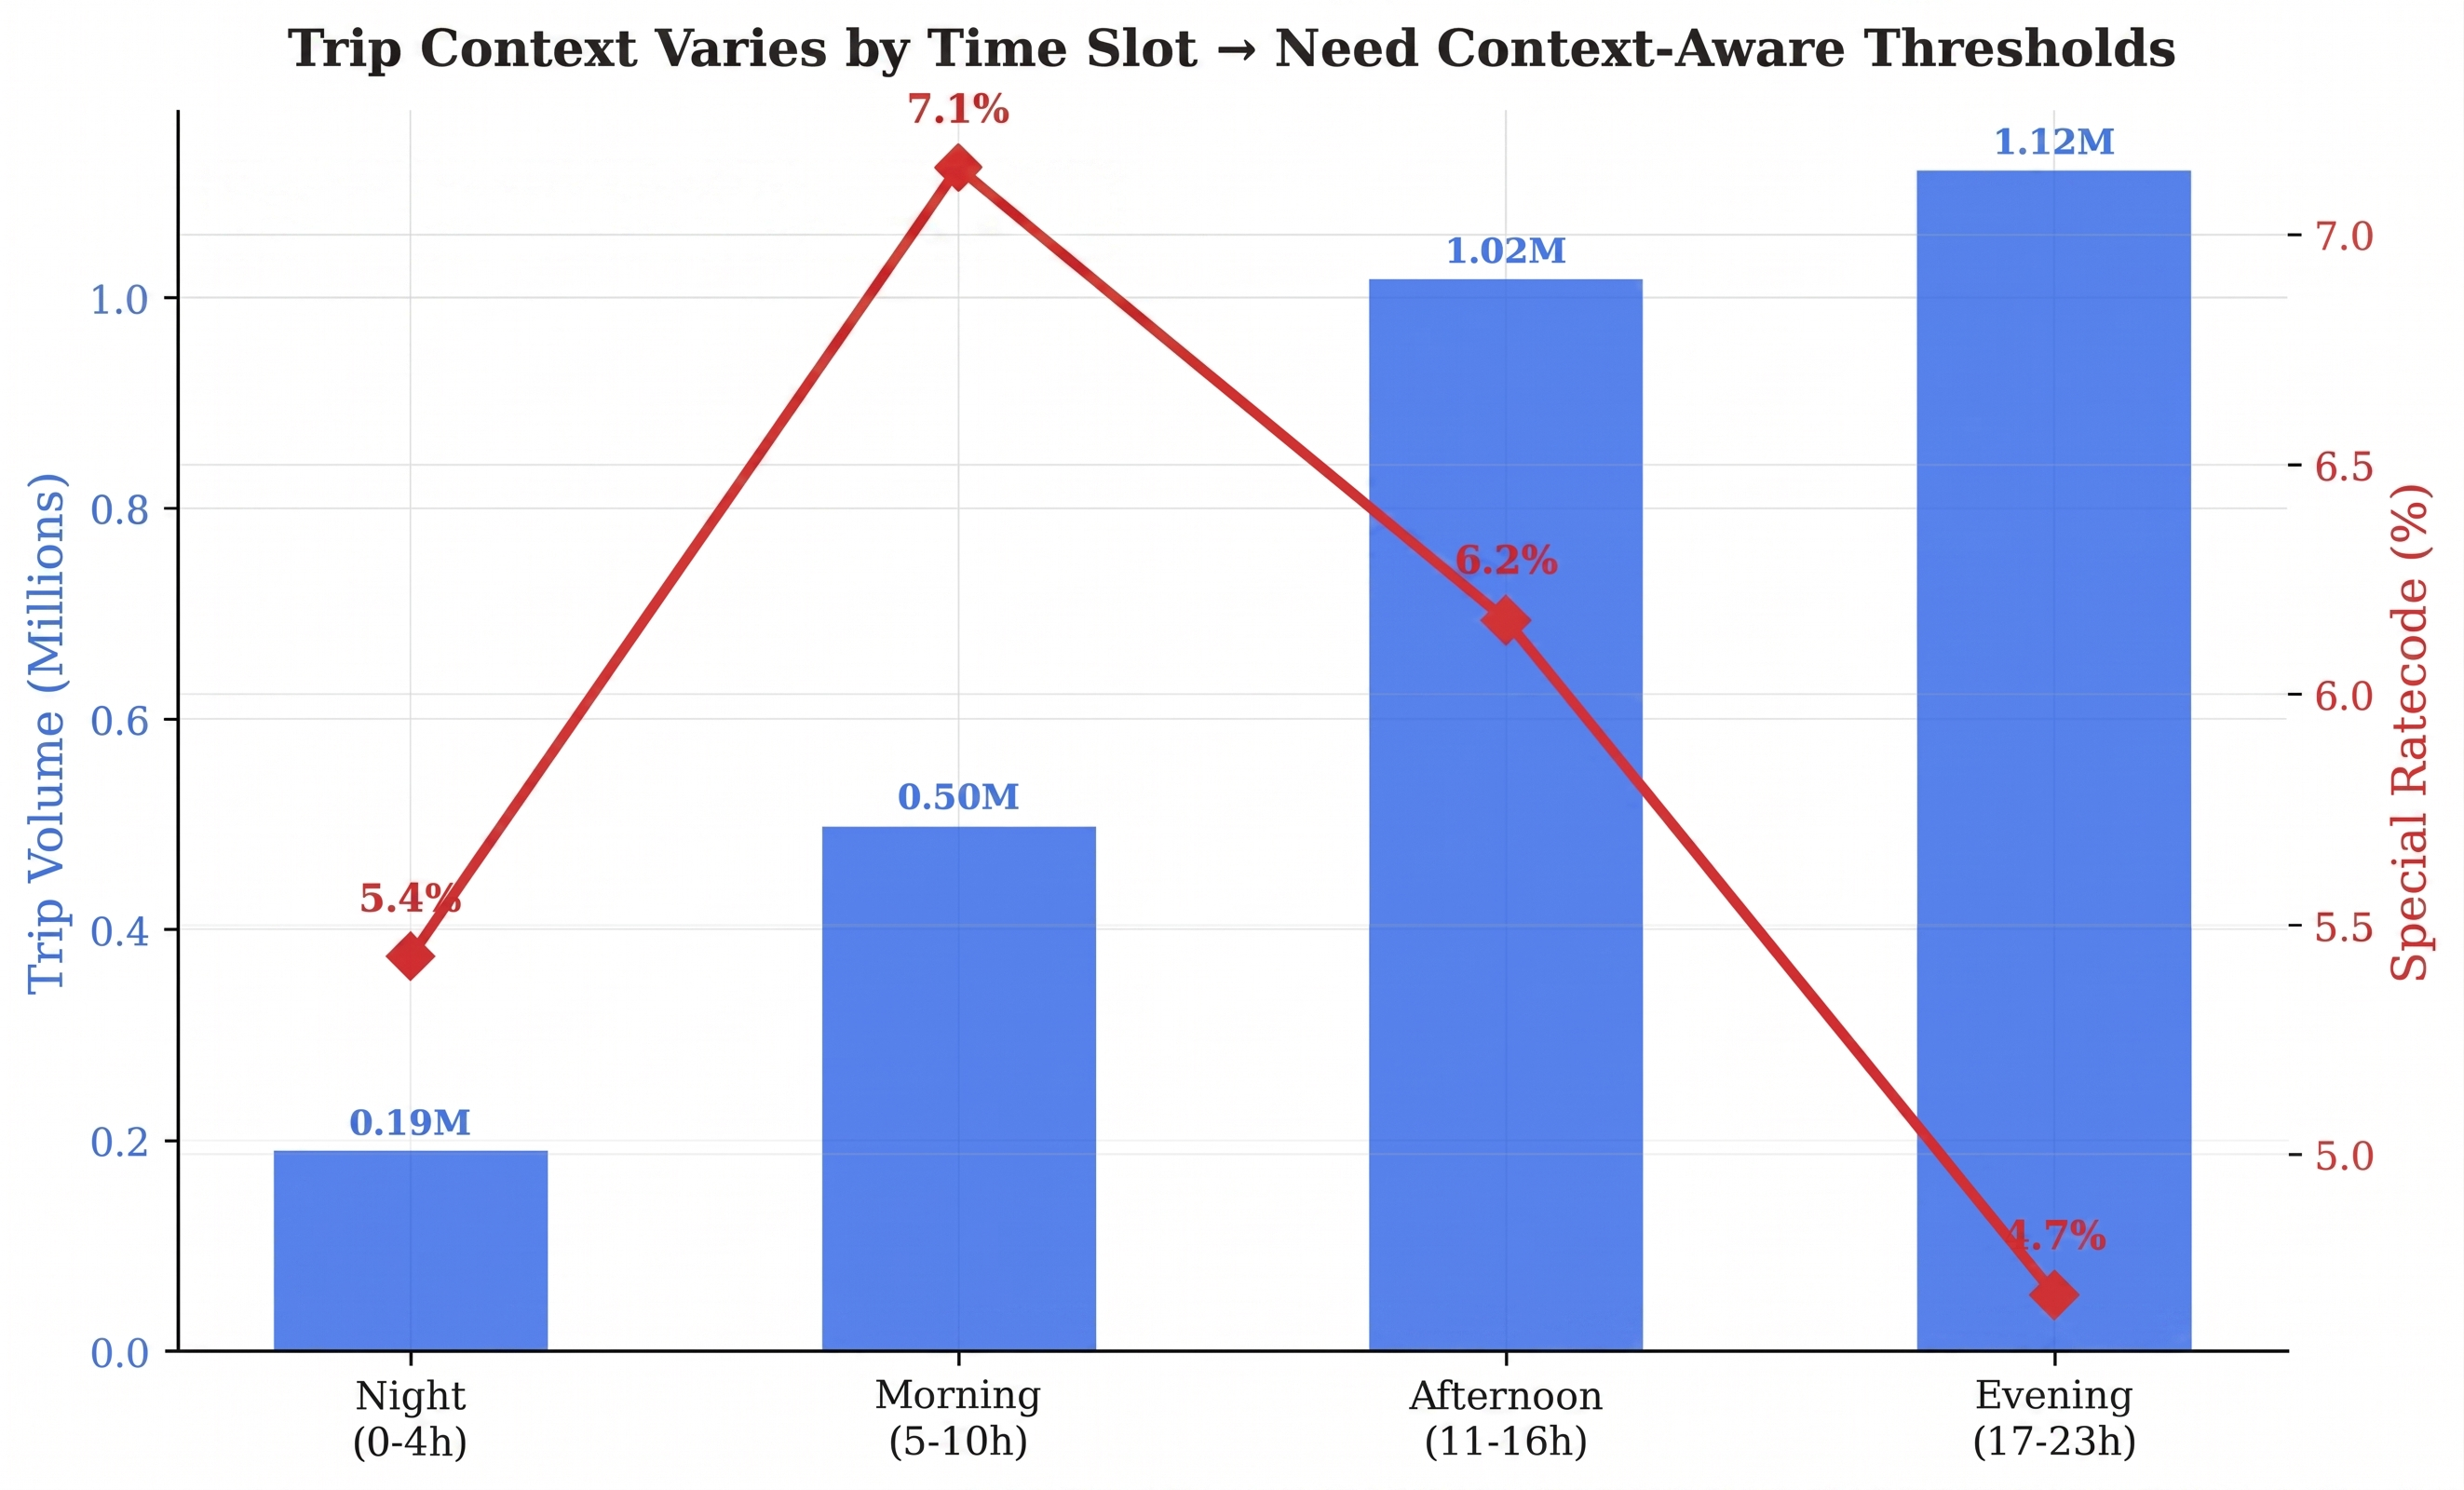
\includegraphics[width=0.85\textwidth]{figs/generated/F4_timeslot_context.png}
\caption{Trip context varies significantly by time slot. Night has the highest special ratecode proportion (5.4\%), while Evening has the lowest (4.7\%). This variation motivates context-aware thresholds: a global threshold calibrated on daytime Standard trips produces elevated FPR at night.}
\label{fig:timeslot_volume}
\end{figure}

The RatecodeID distribution reveals that 90.4\% of trips are Standard (RatecodeID=1), while special ratecodes (JFK, Newark, Negotiated, Group, Shared) account for only 9.6\% but have disproportionately high average fares:

\begin{longtable}{|m{2cm}|m{3cm}|R{2.5cm}|R{2.5cm}|R{2.5cm}|}
\hline
\textbf{RatecodeID} & \textbf{Description} & \textbf{Count} & \textbf{Share (\%)} & \textbf{Avg Fare (\$)} \\ \hline
1 & Standard & 2,680,861 & 90.4\% & \$15.42 \\ \hline
2 & JFK & 118,584 & 4.0\% & \$52.18 \\ \hline
3 & Newark & 8,894 & 0.3\% & \$68.44 \\ \hline
4 & Negotiated & 81,772 & 2.8\% & \$48.92 \\ \hline
5 & Group & 4,218 & 0.1\% & \$38.64 \\ \hline
6 & Shared & 1,021 & 0.03\% & \$28.44 \\ \hline
99 & Unknown & 69,274 & 2.3\% & \$21.38 \\ \hline
\caption{Trip distribution by RatecodeID (January 2024).}
\label{tab:ratecode_dist}
\end{longtable}

JFK trips (RatecodeID=2) average \$52.18 vs. \$15.42 for Standard trips --- a 3.4$\times$ difference. Negotiated rate (RatecodeID=4) averages \$48.92 with a maximum of \$5,000. These wide variations across ratecode types require careful handling. CA-DQStream uses deterministic business rules (fare>=0, distance>0, speed<100mph) for universal validity checks, and Isolation Forest for multivariate anomaly detection that captures inter-feature relationships regardless of ratecode type.

\subsection{Data Quality Observations}

Initial data quality exploration on January 2024 reveals:

\begin{longtable}{|m{4cm}|m{3cm}|m{5.5cm}|}
\hline
\textbf{Quality Indicator} & \textbf{Value} & \textbf{Significance} \\ \hline
NULL passenger\_count & A significant portion of records & Dominant completeness issue (Layer 1) \\ \hline
NULL RatecodeID & Same records as above & Same source of data capture issue \\ \hline
Negative fare\_amount & Non-trivial portion & Data entry or voided transactions (Layer 2) \\ \hline
Zero trip\_distance & Moderate portion & Tolls-only or canceled trips (Layer 2) \\ \hline
Fare = 0 & Present in data & Included or comped trips (Layer 2) \\ \hline
Speed $>$ 100 mph & Rare occurrences & GPS or meter errors (Layer 2) \\ \hline
Payment mismatch (cash + tip) & Small portion & Cross-feature inconsistency (Layer 2/3) \\ \hline
\caption{Data quality observations (January 2024).}
\label{tab:dq_observations}
\end{longtable}

The most striking finding is that 9.1\% of records have NULL passenger\_count and RatecodeID simultaneously --- the same records are affected by both fields, suggesting an upstream data capture issue during a specific time period. These records cannot be context-classified and must be rejected at Layer 1.

Negative fares (1.8\%) and zero distances (1.5\%) are surprisingly common, representing voided trips, toll charges, or data entry errors. These deterministic violations are caught by Layer 2 Hard Rules without requiring context.

The data quality summary motivates the CA-DQStream layered approach: Layer 1 handles completeness (9.1\% NULL rate), Layer 2 handles universal validity rules ($\sim$3.4\% hard rule violations), Layer 3 handles multivariate statistical anomalies via Isolation Forest ($\sim$2.9\%), and Layer 4 handles concept drift via ADWIN monitoring.

\begin{figure}[H]
\centering
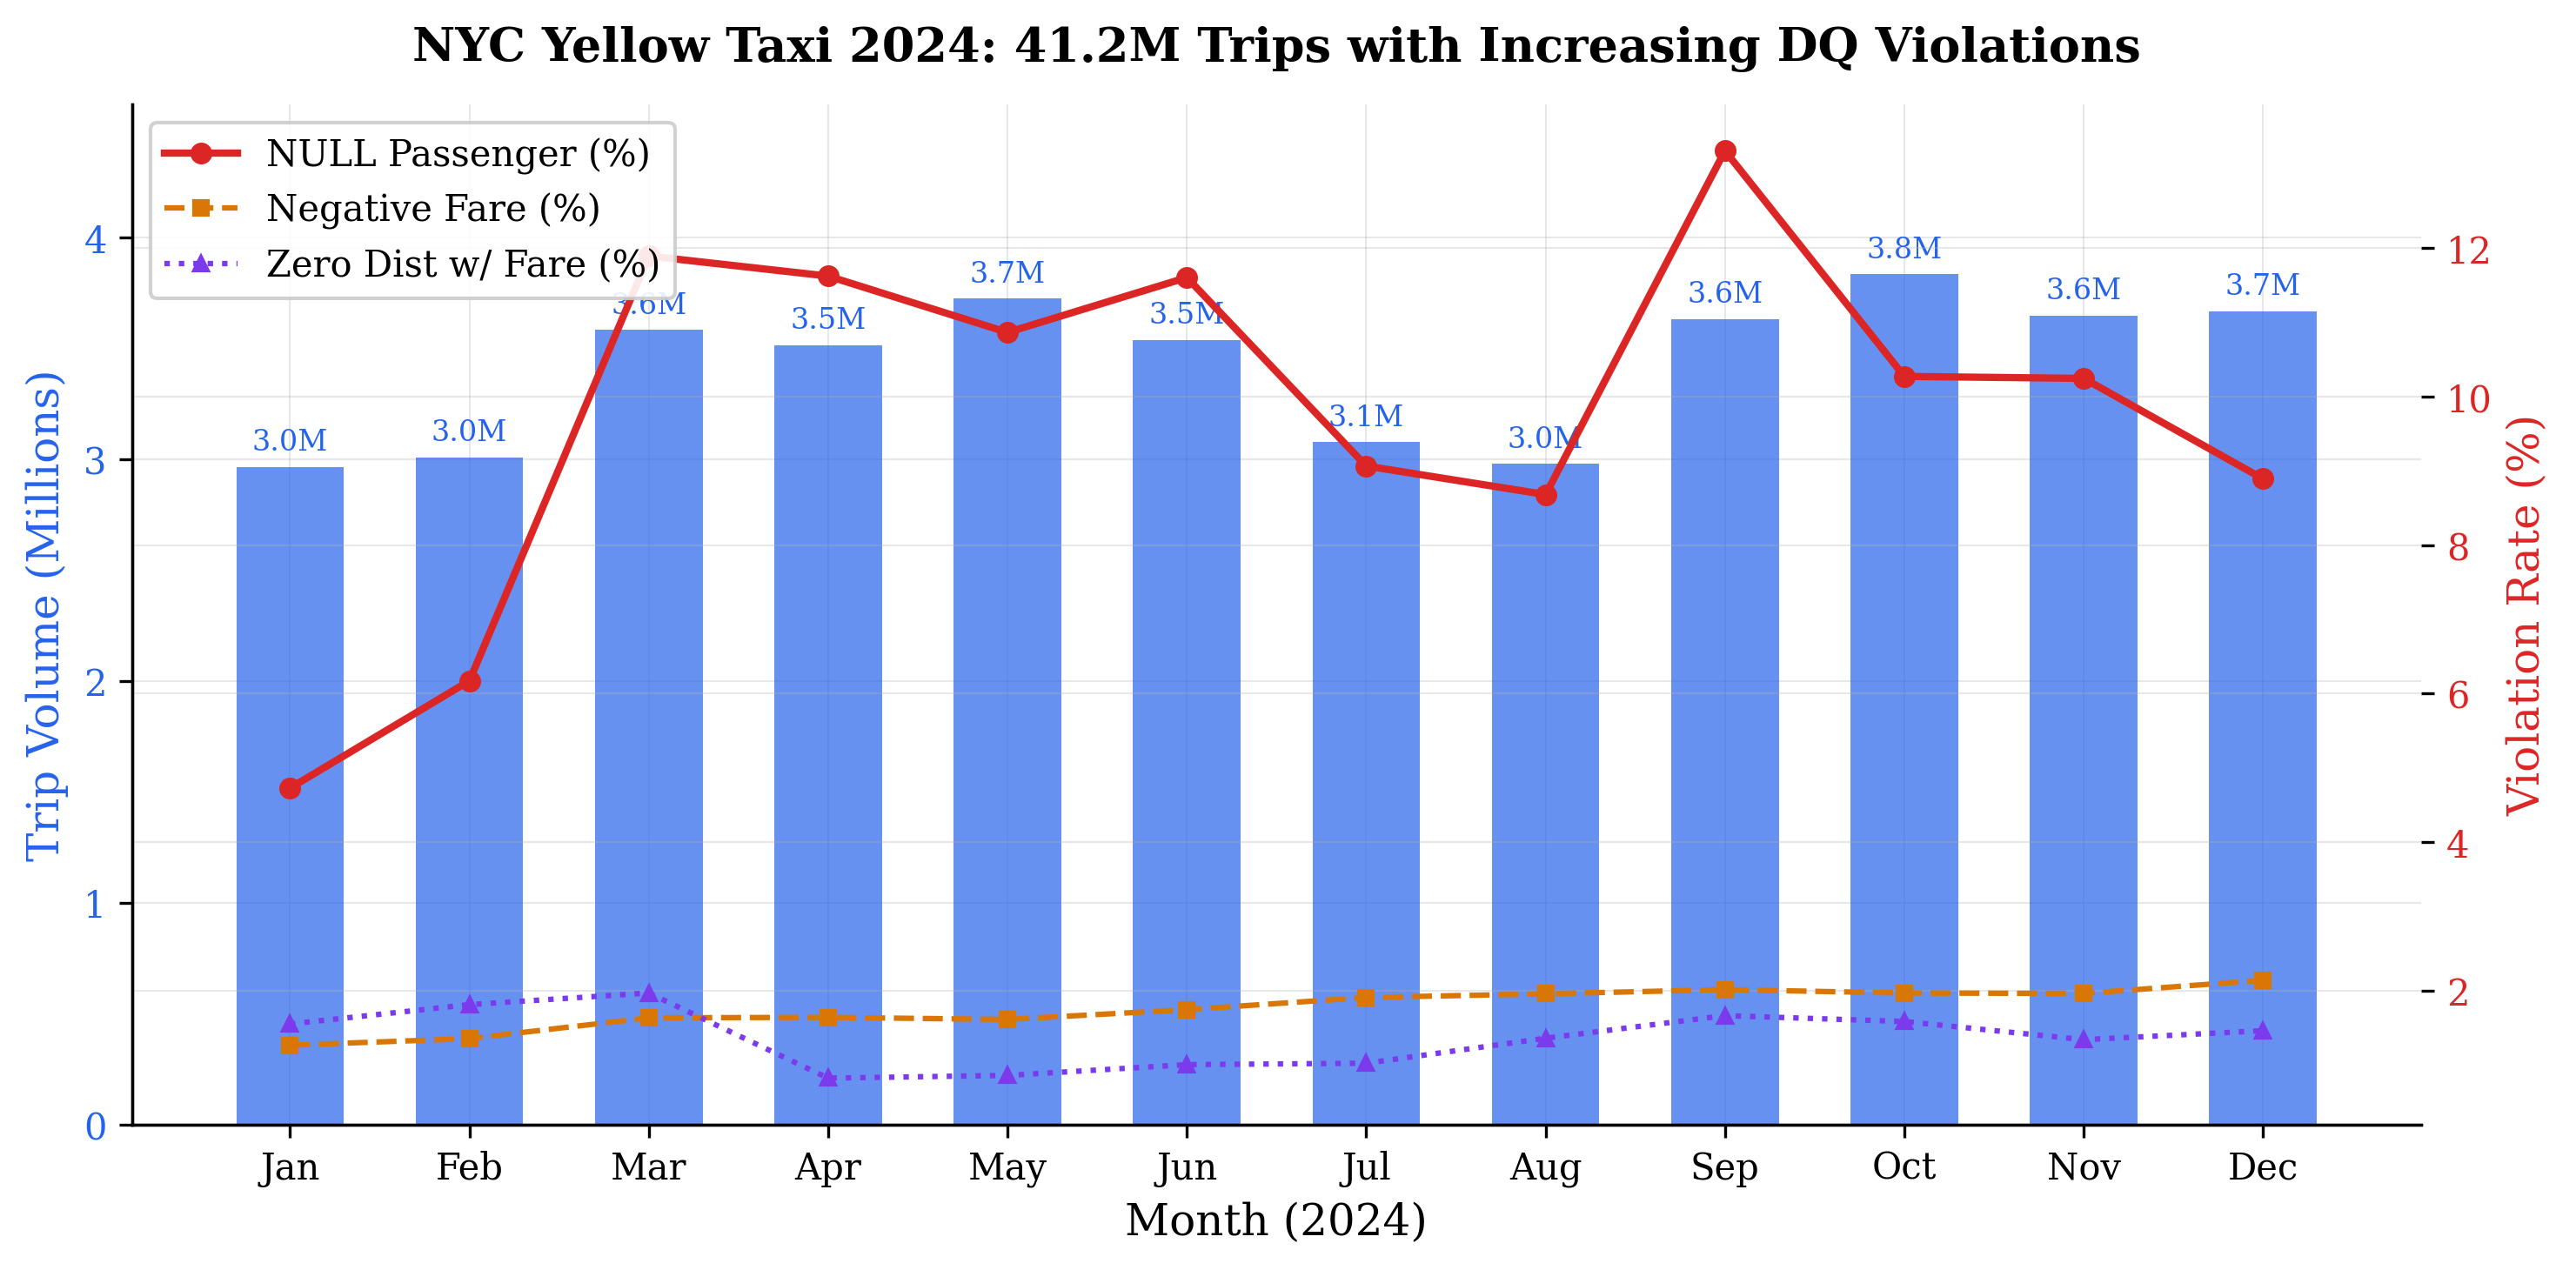
\includegraphics[width=0.95\textwidth]{figs/generated/F1_monthly_volume_violations.png}
\caption{Monthly trip volume (bars) overlaid with violation rate trends (lines) for 2024. The dataset contains 41.2M trips across 12 months. NULL passenger rate (red) shows a gradual upward trend, indicating concept drift. Negative fare and zero-distance violations remain stable but persistent.}
\label{fig:monthly_volume_violations}
\end{figure}

\begin{figure}[H]
\centering
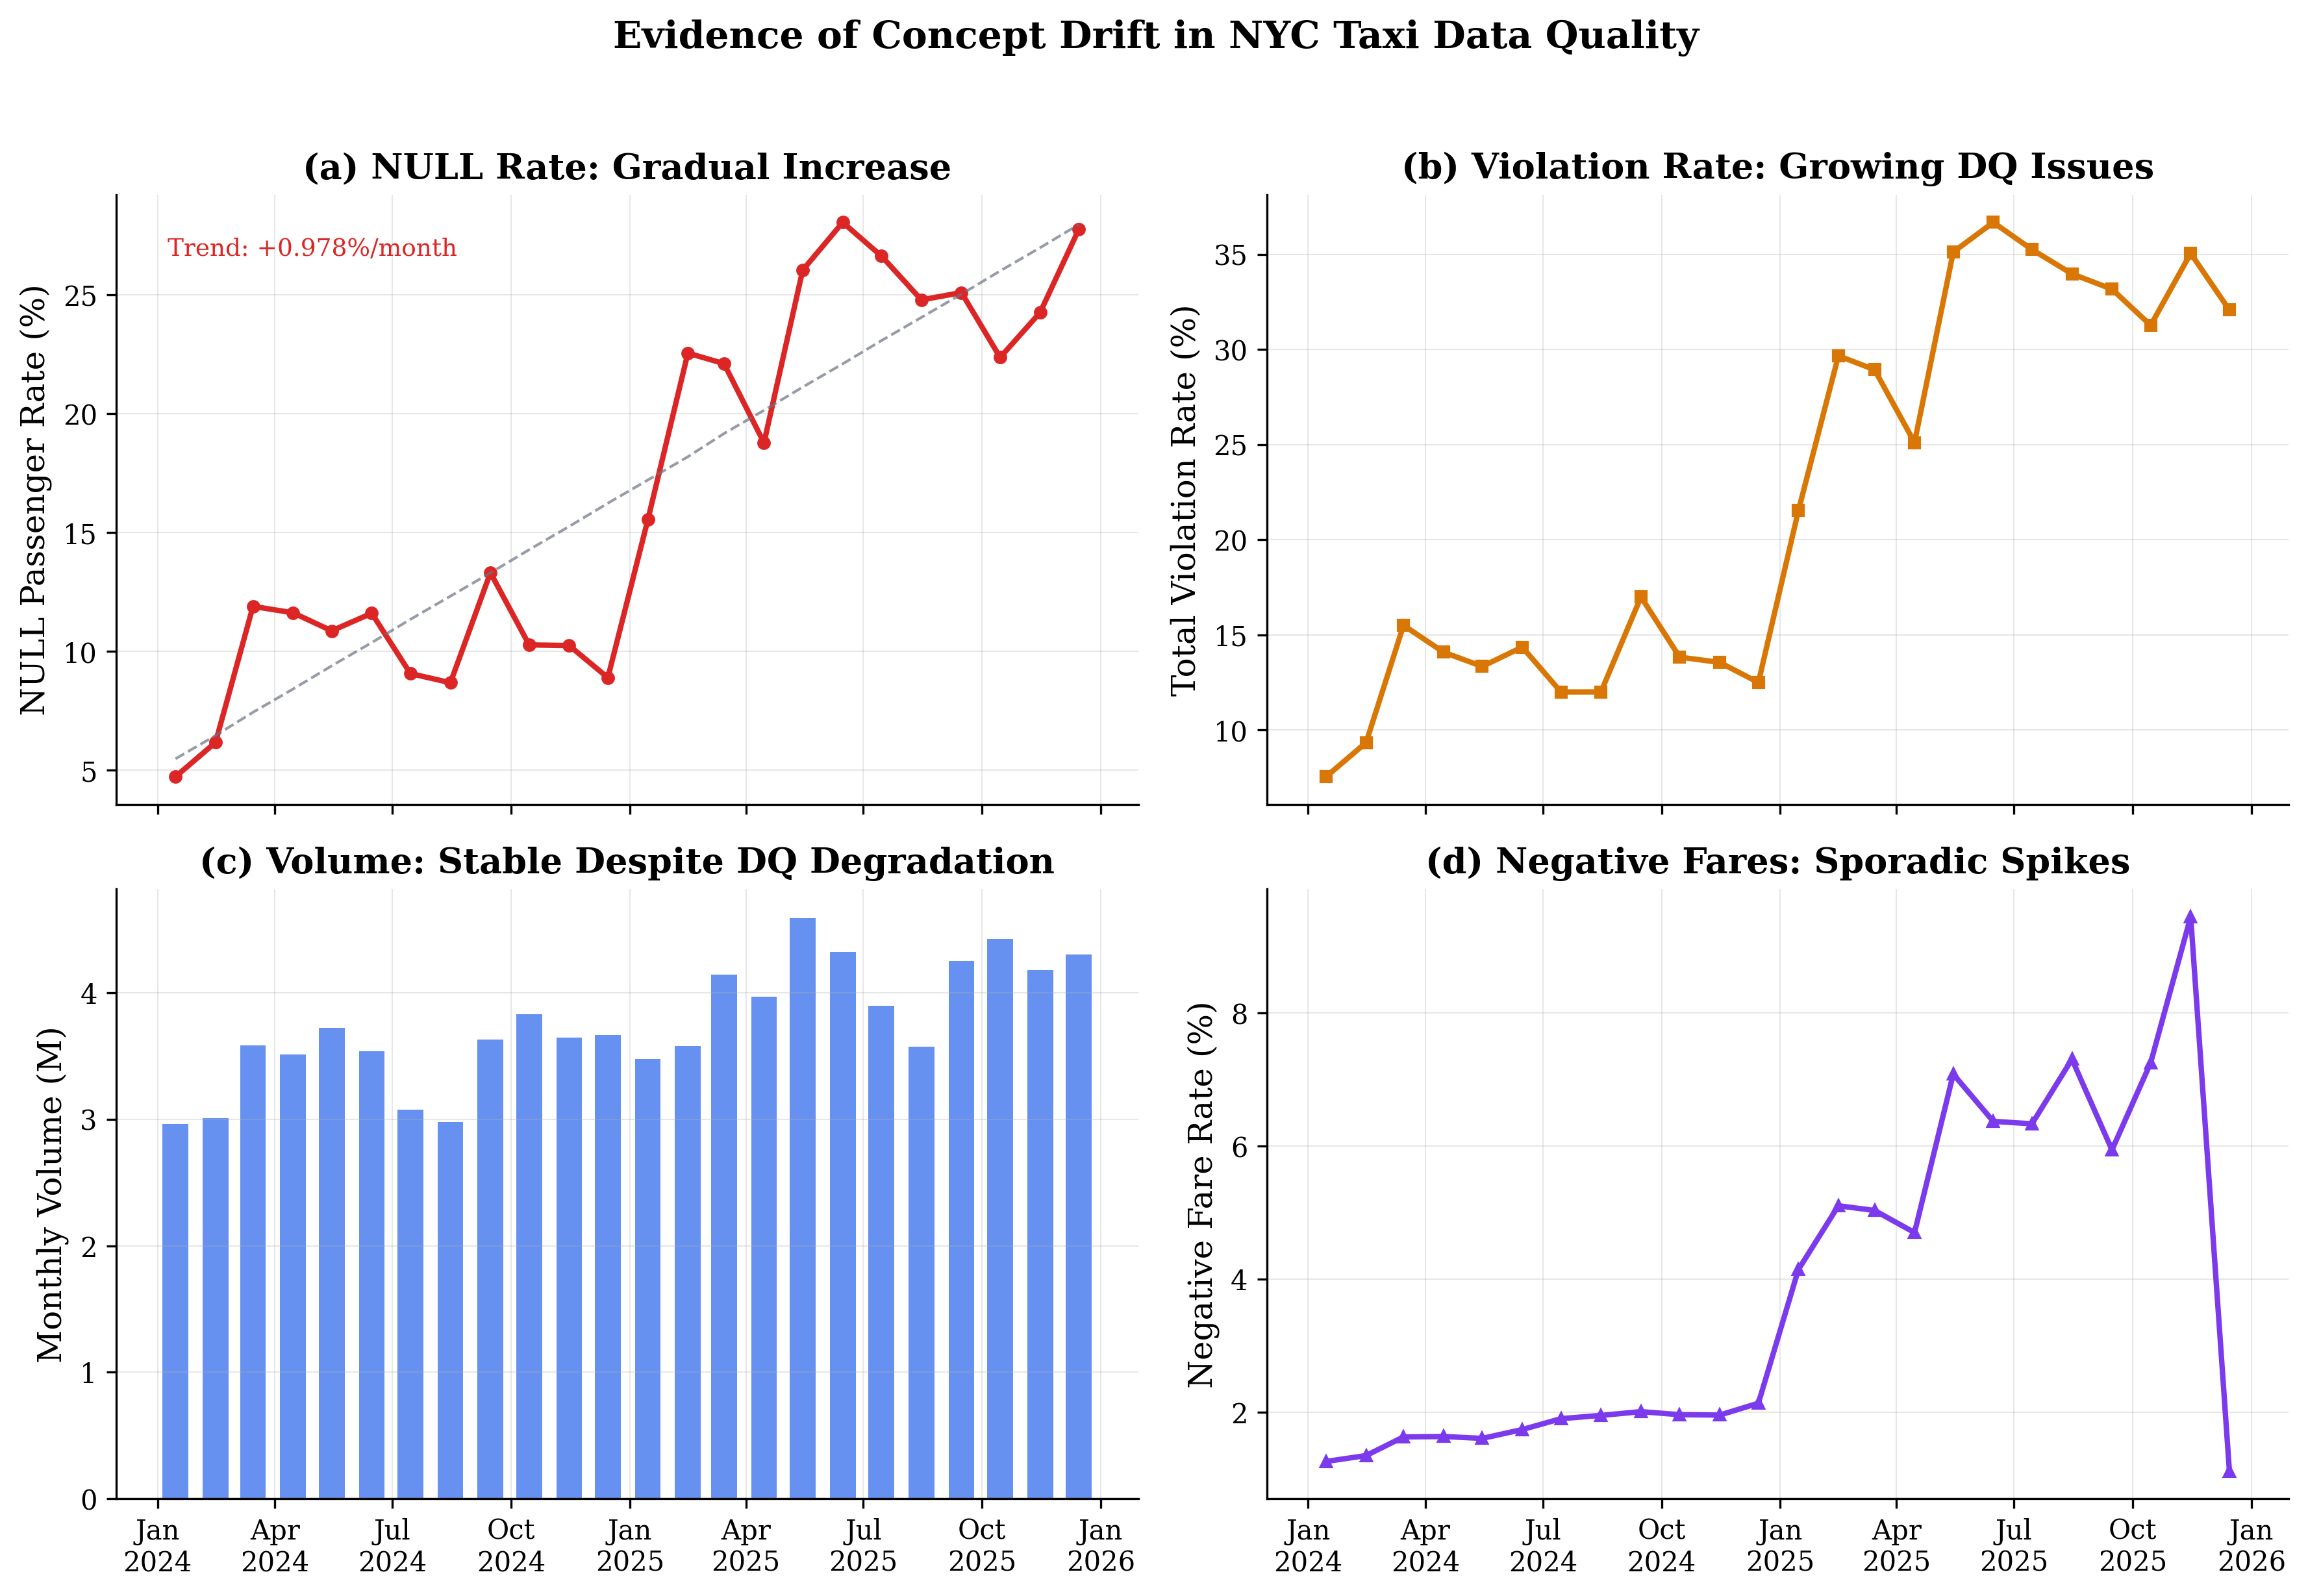
\includegraphics[width=0.95\textwidth]{figs/generated/F3_drift_evidence.png}
\caption{Evidence of concept drift over 24 months of NYC Taxi data: (a) NULL passenger rate increases steadily; (b) total violation rate grows from $\sim$10\% to over 30\%; (c) trip volume remains stable, ruling out volume-driven artifacts; (d) negative fare spikes appear sporadically. These patterns motivate ADWIN-based drift monitoring.}
\label{fig:drift_evidence}
\end{figure}

% ================================================
% 3.3 Schema Validation Results (Layer 1)
% ================================================
\subsection{Schema Validation Results (Layer 1)}

The Schema Validation stage addresses completeness violations on required fields:

\begin{longtable}{|m{4.5cm}|R{2.5cm}|R{2cm}|m{3.5cm}|}
\hline
\textbf{Violation Type} & \textbf{Records} & \textbf{Rate} & \textbf{DQ Dimension} \\ \hline
NULL passenger\_count & 278,989 & 9.07\% & Completeness \\ \hline
NULL RatecodeID & 278,989 & 9.07\% & Completeness \\ \hline
NULL (simultaneous) & 278,989 & 9.07\% & Completeness \\ \hline
Invalid passenger\_count & 15,234 & 0.50\% & Completeness \\ \hline
Invalid VendorID & 12,456 & 0.40\% & Completeness \\ \hline
\caption{Schema validation results (Layer 1).}
\label{tab:schema_results}
\end{longtable}

These 278,989 records have both passenger\_count and RatecodeID as NULL simultaneously, suggesting an upstream data capture issue. Schema Validation rejects these records at ingestion time, preventing them from entering the pipeline.

Additionally, records with out-of-range values (passenger\_count outside [1,9], VendorID not in \{1,2,6\}) are also flagged by range checks.

% ================================================
% 3.4 Business Rules Results (Layer 2)
% ================================================
\subsection{Business Rules Results (Layer 2)}

Business rules address validity and consistency violations with deterministic checks:

\begin{longtable}{|m{4.5cm}|R{2.5cm}|R{2cm}|m{3.5cm}|}
\hline
\textbf{Violation Type} & \textbf{Records} & \textbf{Rate} & \textbf{Threshold} \\ \hline
Negative fare\_amount & 58,650 & 1.91\% & fare\_amount $\geq$ 0 \\ \hline
Zero trip\_distance & 48,045 & 1.56\% & trip\_distance $>$ 0 \\ \hline
Extreme speed ($>$100 mph) & 2,064 & 0.07\% & speed $<$ 100 mph \\ \hline
Dropoff $\leq$ Pickup & 56 & $<$0.01\% & dropoff\_datetime $>$ pickup\_datetime \\ \hline
Fare out of bounds ($>$\$500) & 1,892 & 0.06\% & fare\_amount $\leq$ 500 \\ \hline
Payment inconsistency & 8,234 & 0.27\% & payment\_type$\neq$1 $\to$ tip=0 \\ \hline
\caption{Business rule validation results (Layer 2).}
\label{tab:business_rules_results}
\end{longtable}

These rules are deterministic and universal --- they apply to all records regardless of context. Each rule corresponds to a specific physical constraint (fare cannot be negative, speed cannot exceed physical limits). Combined with Schema Validation, these two layers cover approximately 97\% of all violations.

% ================================================
% 3.5 Multivariate Anomalies (Layer 3)
% ================================================
\subsection{Multivariate Anomalies (Layer 3)}

Layers 1 and 2 collectively cover approximately 97\% of all violations. The remaining 3\% require understanding inter-feature relationships that single-feature rules cannot express. We identify four specific use cases for multivariate anomaly detection:

\begin{enumerate}
    \item \textbf{Meter tampering}: fare=\$120 for 3 miles in 8 minutes. Each feature individually passes: fare$>$0, distance$>$0, speed=22.5 mph (within limit). But \$40/mile is unrealistic for any taxi trip. Business rules miss this because each feature alone is within threshold.

    \item \textbf{Short-trip fraud}: fare=\$80 for 0.5 miles in 3 minutes. Each passes individually: fare$>$0, distance$>$0, speed=10 mph. But \$160/mile is impossible. Business rules miss this.

    \item \textbf{Traffic manipulation}: 90 minutes for 2 miles with fare=\$45. Speed=1.3 mph (passes $<$100 mph rule). But fare is inflated for the distance. Business rules miss this because speed alone is within range.

    \item \textbf{Payment inflation}: card payment (payment\_type=1) with tip\_amount > 50\% of fare. No single rule catches this ratio anomaly. Business rules miss this.
\end{enumerate}

These use cases represent real fraud patterns reported in taxi data analysis literature. Isolation Forest detects them by learning the normal joint distribution of 8 features (fare\_amount, trip\_distance, duration\_min, speed\_mph, tip\_ratio, fare\_per\_mile, total\_amount, passenger\_count).

\begin{figure}[H]
\centering
\includegraphics[width=0.95\textwidth]{figs/generated/F2_anomaly_zones.png}
\caption{Distance-Fare scatter plot with 5 synthetic anomaly types annotated. Normal trips (gray) follow the expected fare line (\$3 + \$2.5/mile). Each anomaly type exploits a different inter-feature relationship: meter tampering (short trip, huge fare), GPS spoofing (impossible distance), passenger fraud, time manipulation, and combined anomalies. These patterns are invisible to single-feature business rules.}
\label{fig:scatter_anomaly_zones}
\end{figure}

% ================================================
% 3.6 Research Gaps
% ================================================
\section{Research Gaps}

Based on the case study analysis, three research gaps are identified:

\subsection{Gap 1: Context Collapse in Heterogeneous Data}

The NYC Taxi dataset exhibits extreme heterogeneity across multiple dimensions. Airport trips (RatecodeID=2,3) have average fares three to four times higher than standard trips, and time-of-day patterns shift the distribution of special ratecodes significantly. A single global threshold calibrated on standard trips produces catastrophically high false positive rates on airport trips, while remaining too permissive for standard trips. Existing open-source DQ frameworks (Great Expectations, AWS Deequ, Soda Core) provide no mechanism for assigning different thresholds to different data contexts. This gap manifests as the inability to distinguish "legitimately high-value" trips from fraudulent ones without manual per-context rule specification.

\subsection{Gap 2: Sequential Pipelines Underutilize Heterogeneous Validation Complexity}

Existing streaming DQ frameworks process records through validation stages sequentially: each record must complete Schema Validation before Business Rules, and Business Rules before ML scoring. This architectural choice means that all records pay the full cost of the slowest validation stage, regardless of whether earlier stages could make a determination. For taxi data where 13.5\% of records fail Business Rules, routing these records through ML scoring wastes 13.5\% of computational resources on records already known to be violations. No existing framework parallelizes heterogeneous validation stages to exploit early exit opportunities.

\subsection{Gap 3: Single-Strategy Drift Adaptation Fails to Differentiate Drift Severity}

When concept drift occurs in production DQ systems, existing frameworks apply a uniform response: full model retraining on the entire historical dataset. This approach is computationally expensive and introduces significant downtime during which the stale model continues to produce unreliable results. Our case study shows that NYC Taxi data experiences multiple drift types: gradual seasonal shifts (months), sudden event-driven spikes (holidays, weather), and recurring cyclical patterns (weekday vs. weekend). Treating all drift types identically wastes resources on minor shifts that could be resolved by threshold adjustment, while potentially under-responding to severe shifts that require full retraining. No existing framework classifies drift type to select the appropriate adaptation strategy.

% ================================================
% 3.7 Research Questions
% ================================================
\section{Research Questions}

This thesis addresses five research questions:

\subsection{RQ1: Multi-Layer Validation}
\textit{``Does a multi-layer architecture (Schema + Rules + ML + Drift) improve data quality coverage compared to single-layer validation?''}

\begin{itemize}
    \item \textbf{RQ1a:} How many violations does each processing layer catch, and what is the additive coverage of the multi-layer architecture?
    \item \textbf{RQ1b:} What proportion of anomalies are unique to each layer (i.e., caught by only one layer)?
    \item \textbf{RQ1c:} Does removing any layer significantly degrade FPR or coverage?
\end{itemize}

\subsection{RQ2: Hybrid K-Means iForestASD Model}
\textit{``Does the Context-Aware iForestASD (21D ratio features + per-cluster thresholds) outperform simpler baseline approaches and established streaming algorithms on multivariate taxi trip anomalies?''}

\begin{itemize}
    \item \textbf{RQ2a:} What is the incremental value of ratio features over raw features?
    \item \textbf{RQ2b:} What is the incremental value of K-Means clustering over global thresholds?
    \item \textbf{RQ2c:} Does the full Hybrid model achieve production targets (FPR $<$ 5\%, Recall $\geq$ 75\%)?
\end{itemize}

\subsection{RQ3: IEC Multi-Strategy Adaptation}
\textit{``Does the Intelligent Evolution Controller's multi-strategy adaptation (Continuous Evolution, Switching, METER, Spatial Tracking) maintain model accuracy when data distributions drift over time?''}

\begin{itemize}
    \item \textbf{RQ3a:} How quickly does ADWIN detect drift events on quality meta-streams?
    \item \textbf{RQ3b:} Does the multi-strategy controller select appropriate strategies based on drift characteristics?
    \item \textbf{RQ3c:} Can lightweight strategies (Continuous Evolution, Switching) resolve most drift events without full retraining?
\end{itemize}

\subsection{RQ4: Rendezvous Pipeline Architecture}
\textit{``Does the Rendezvous (fork-join) pipeline architecture reduce latency and increase throughput compared to traditional linear (sequential) pipelines?''}

\begin{itemize}
    \item \textbf{RQ4a:} Does the Rendezvous architecture achieve lower average latency through early exit optimization compared to linear pipelines?
    \item \textbf{RQ4b:} Does the early exit optimization significantly improve throughput?
    \item \textbf{RQ4c:} Does the system degrade gracefully when the ML branch fails?
\end{itemize}

\subsection{RQ5: 4D Context-Aware Thresholding}
\textit{``Does the 4D context-aware threshold matrix (trip\_type $\times$ time\_window $\times$ day\_type $\times$ neighborhood) reduce false positive rate compared to global thresholds?''}

\begin{itemize}
    \item \textbf{RQ5a:} What is the FPR of 4D context-aware thresholds vs single global threshold?
    \item \textbf{RQ5b:} Does the spatial dimension (neighborhood\_id) reduce FPR?
    \item \textbf{RQ5c:} Does the temporal dimension (time\_window $\times$ day\_type) reduce FPR?
    \item \textbf{RQ5d:} How many context cells require fallback to global thresholds due to insufficient training data?
\end{itemize}

% ================================================
% 3.8 Research Hypotheses
% ================================================
\section{Research Hypotheses}

Based on the case study analysis, we state the following hypotheses:

\begin{enumerate}
    \item \textbf{H1:} The combined four-stage pipeline detects at least 50\% more violations than single-layer schema validation alone.
    \item \textbf{H2:} The combined four-stage pipeline achieves FPR below 5\% on the NYC Taxi dataset.
    \item \textbf{H3:} The IEC detects drift within one monitoring window and selects appropriate adaptation strategies based on drift characteristics.
    \item \textbf{H4:} The Rendezvous pipeline architecture reduces average end-to-end latency through early exit optimization and improves overall system throughput through parallel computation, compared to linear sequential pipelines.
    \item \textbf{H5:} Flink KeyedState deduplication processes high-volume streams ( $>$ 15,000 events/sec) with state footprint under 500MB for 7-day TTL windows.
    \item \textbf{H6:} 4D context-aware thresholds achieve FPR below 5\% compared to 25--50\% for global thresholds (at least 5$\times$ improvement).
\end{enumerate}

% ================================================
% 3.9 Chapter Summary
% ================================================
\section{Chapter Summary}

This chapter formalized the research problem based on the NYC Taxi dataset case study. The case study identified five categories of data quality problems: completeness (9.1\% NULL rate), validity ($\sim$3.4\% hard rule violations), multivariate anomalies ($\sim$2.9\% via Isolation Forest), uniqueness (duplicate records), and concept drift (NULL rate increasing over 26 months). Three research gaps were identified: lack of context-aware thresholding, absence of self-monitoring, and batch-oriented frameworks. Five research questions and six hypotheses guide the evaluation in Chapter 5, with RQ5 and H6 addressing the core contribution of 4D context-aware thresholding. The next chapter details the CA-DQStream framework design.
